\subsection{User Taxonomy based on Peak Ratio}
\label{subsec:peakratio}
% the ratio of the 90\%-ile to the median throughput per day.

\begin{figure}[ht!]
\begin{minipage}{0.90\linewidth}
\centering
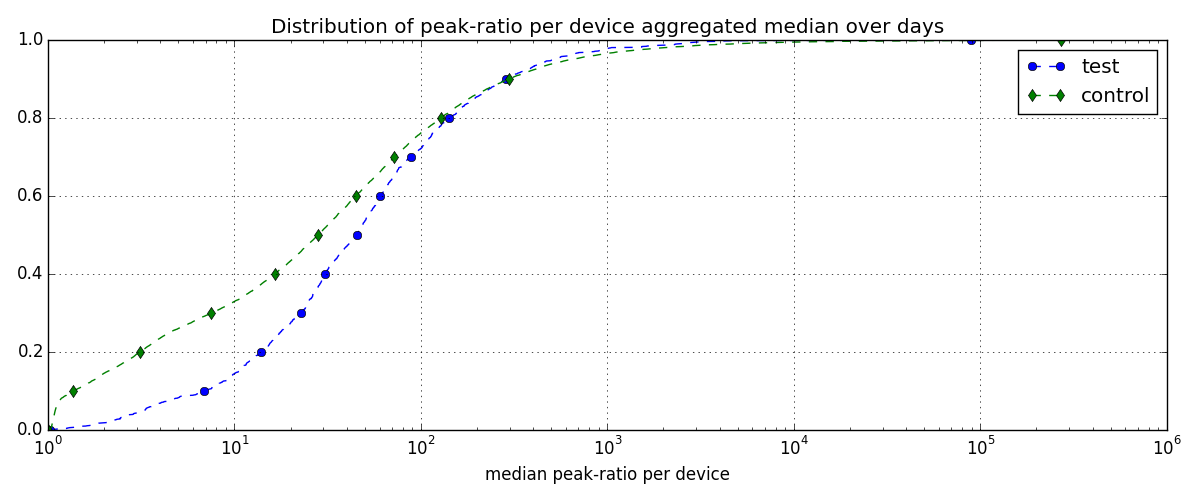
\includegraphics[width=1\linewidth]{figures/peakratio-CDF-devices-MEDIAN.png}
\caption{Median peak ratio per device showing that test set has higher daily ratio (50 times by median). Thus ISPs should condition their networks to 50 times the median usage for each user added in the worst case scenario.}
%http://sites.noise.gatech.edu/~sarthak/files/comcast/plots/full_dw/peakratio-CDF-devices-MEDIAN.png
\label{fig:CDF-peak-ratio-median}
\end{minipage}
\end{figure}

\paragraph{Peak Ratio: }To further characterize and compare the deviation of data rate for the \control and \test set, we examine \emph{peak-ratio} as defined in ~\ref{sec:methodology} 
Figure ~\ref{fig:CDF-peak-ratio-median} shows that the median peak-ratio for each device in the \test set is much larger than that of the \control set.
\todo{replace much larger with the exact number or percentage}.
\sg{Taken together} with our observations of a lower prime-time ratio of the \test set (section~\ref{subsec:primetime}) this implies that there are households in the \test set that achieve a peak-ratio $>$ 1, but not during the prime-time hour. We believe that these households might actually be small businesses or work-at-home users that peak during daytime hours instead of evening hours.

\begin{figure}[ht!]
\begin{minipage}{0.9\linewidth}
\centering
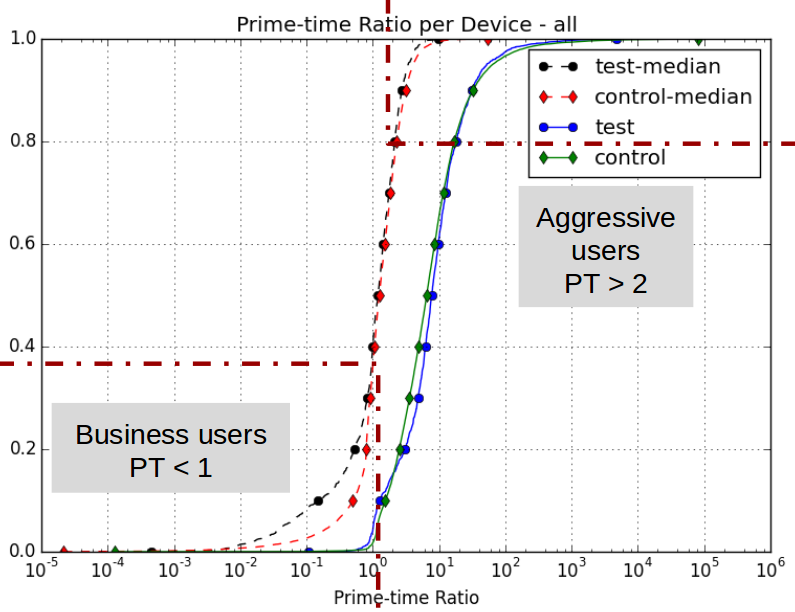
\includegraphics[width=0.9\linewidth]{figures/cdf-prime-time-ratio[replace].png}
\caption{(old) Prime Time ratio + usage can be used to divide users into four sets: aggressive all time + non aggressive all time, aggressive peak time, aggressive non-peak time (business hours). 30\% PT $<$ 1: possibly businesses with normal work-hours . 20\% PT $>$ 2: aggressive prime-time streamers}
%http://riverside.noise.gatech.edu:8083/separated/full/cdf-prime-time-ratio-per-device.png\\
%http://riverside.noise.gatech.edu:8083/plots/full_dw/prime-time-ratio-per-device-cdf-ALL.png
\label{fig:CDF-prime-time-ratio}
\end{minipage}
\end{figure}

The median peak-ratio per device itself shows a large range, from 1 to 10e6 (figure~\ref{fig:CDF-peak-ratio-median}), and the maximum peak-ratio per device was an order higher. Clearly there are some households that have a very even usage throughout the day (low peak ratio), and others that are extremely aggressive only at certain times (high peak ratio). We plot this segregation in figure ~\ref{fig:CDF-prime-time-ratio}.

\todo{EVERYTHING BELOW THIS IS TODO}

\paragraph{User Taxonomy:} The Sandvine reports present a taxonomy of users based on their contribution to real-time entertainment traffic. We incorporate a similar definition based on contribution to data traffic, along with our observations of utilization, to present a taxonomy of the users in our dataset. One category of users is the non-utilizers, i.e., non-aggressive low bandwidth users, that contribute less than SOME THRESHOLD PERCENTILE to the daily data transferred \sg{these the ISP can ignore, also they probably don't need this tier as their utilization from the previous section must be super low}. The second category is of users contributing most aggressively to the data at the ISP \sg{these users will probably gobble up a higher capacity link if given a chance - they're the ones who effect all our graphs.. Need to check this claim}. We further subdivide this high utilizing subcategory based on differing prime-time ratio and peak-ratios follows... \todo{need to think and analyze this further: technical definition to do the analysis}
\begin{itemize}
\item Aggressive All-Time: Users having a low peak-ratio due to a lower variance. Is also expected to have a low prime-time ratio.
\item Aggressive Prime-Time: The usual streamer with a high prime-time ratio and a high peak ratio.
\item Aggressive Non-Prime-Time: Possibly a business user with a low prime-time ratio  but a high peak ratio
\end{itemize}

% other results:
%big difference (2 x median ratio) in per device per day ratios of 90%ile:median.
%weird shape again for values < ratio 100
%big difference in this ratio per day, and it is consistent across all individual sets + months.
%very large for Dec, slightly smaller for Nov
%interestingly, at higher ratios control is slightly > test. This means that certain devices in control set have a huge std (ratio) in a day as compared to test set which has a lower “max” ratio.

\todo{ TO PLOT :}
\begin{itemize}
\itemsep0em
\item peak ratio cdf vs no of devices
\item peak ratio cdf vs time of day where peak occurred
\item no of devices cdf vs time of day where peak occurred
\end{itemize}

Based on differing usage profiles within the same high tier bandwidth, we suggest that the FCC adopt multiple benchmarks based on usage characteristics to better characterize broadband availability, deployment, and adoption in the US. Such multiple benchmarks can be the minimum broadband speed required per user based on the kind of traffic expected during a day. ISPs can also offer these users better plans based on hour-of-the-day or usage caps to encourage more off-peak usage. These users probably don't cause latency spikes in PT.


We recommend multiple standards...